\section{Evaluation}\label{sec:evaluation}
The evaluation focuses on computations that are expected to profit from parallelization, e.g. compute-intensive tasks or tasks over a large set of data. However, using the presented runtime system may also be beneficial for long-running, but not parallelized computations that otherwise would block the main thread and result in a degraded user experience. The evaluation compares the presented work with the alternatives introduced in \cref{sec:related-work} concerning performance and applicability to the following set of problems:

\begin{itemize}
	\item[$\bullet$] Knight Tour: Computes the number of open tours from a given start field. Low memory usage but very high computational needs.
	\item[$\bullet$] Mandelbrot $10'000 \times 10'000$: Computation of a Mandelbrot for a given image size. This problem requires a relatively large amount of memory compared to the computational time needed.
	\item[$\bullet$] Risk Profiling: The risk profiling uses a Monte Carlo simulation to create forecasts for the customer's asset development over a period of 15 years for various investment strategies and assuming different states of the economic. The forecast is used to explain to the customer how the chosen investment strategy and the state of the economic effects the development of his assets and therefore, planned investments --- e.g. buying a house after ten years. This problem is an instance of a real-world problem~\cite{Kwsoft2016}.
\end{itemize}

The versions of the runtime systems used used by the evaluated are shown in \cref{tab:runtime-system-version}.

\begin{table}
	\centering
	\begin{tabular}{p{0.6\linewidth} l}
		\toprule
		Runtime System & Version \\ \midrule
		Parallel.es & 0.1.17 \\
		Hamsters.js & 3.9.0\footnote{The version used is based on 3.9.0 but contains a fix for input data that is not a typed array (\url{https://github.com/austinksmith/Hamsters.js/issues/16}).} \\
		Parallel.js & 0.2.x\footnote{Latest version from master as mentioned in \cref{sec:related-work}.} \\
		Threads.js & 0.7.2 \\ \bottomrule
	\end{tabular}
	\caption{Versions of Evaluated Runtime Systems}
	\label{tab:runtime-system-version}
\end{table}


\subsection{Applicability}
The applicability is mainly evaluated by comparing the Mandelbrot implementations. The synchronous, lodash~\cite{lodash} based implementation of the Mandelbrot has been introduced in \cref{sec:programming-model} and is shown in \cref{fig:mandelbrot-sync}. The implementation to compute a single pixel is omitted for brevity since it is almost identical for all evaluated runtime system. The preliminary focus of the evaluation is on readability and type-safety. However, some of the results might be subjective and represent the opinion of the author. 

\paragraph{Parallel.es}
\Cref{code:mandelbrot-parallel.es} from \cref{sec:programming-model} shows the Mandelbrot implementation using Parallel.es. The implementation is almost identical to the synchronous, lodash~\cite{lodash} based implementation shown in \cref{fig:mandelbrot-sync}. This similarity of the APIs facilitates a fast learning curve and simplifying the adoption of existing code. The API of Parallel.es is type-safe for a seamless integration into projects developed with typed languages. The programming model of Parallel.es allows task functions to reference functions and read-only variables from its outer scope giving the programmer the liberty to structure the code as he desires and not according to the requirements of the runtime systems. This freedom allows a seamless integration of parallel task that none of the other evaluated runtime systems achieves. However, this liberty comes at the cost that the source code needs to be transpiled what potentially requires an additional build step. The author believes that the benefits of a seamless integration outweigh the additional complexity in the build process. Especially because transpiling of source code --- mostly using Babel~\cite{babel} --- is very common in the JavaScript community. 

\paragraph{Parallel.js}
\Cref{fig:mandelbrot-paralleljs} shows the Mandelbrot implementation using the reactive API of Parallel.js. It differs only slightly from the synchronous implementation. A parallel task is created using the \javascriptinline/Parallel/ constructor (line \ref{code:paralleljs-definition}). The first constructor argument is the data to process, the second --- optional --- is an options object affecting the task execution where the value of the \javascriptinline/env/ property is exposed as \javascriptinline/global.env/ in the background thread (line \ref{code:paralleljs-global}). The task function passed to the \javascriptinline/map/ operation (line \ref{code:paralleljs-map}) is called for every element in the input array and produces the elements in the output array.

\begin{listing}
	\begin{javascriptcode*}{highlightlines={9, 22-29}}
const imageWidth = 10000;
const imageHeight = 10000;

function computePixel(x, y) {
	// ...
	return n;
}

function computeMandelbrotLine(y, imageWidth) {
	const arraySize = imageWidth * 4;
	const line = new Uint8ClampedArray(arraySize);
	
	for (let x = 0; x < imageWidth; ++x) {
		line[x * 4] = computePixel(x, y);
	}
	
	return line;
}

const lines = _.range(imageHeight);

new Parallel(lines, {env: { imageWidth } }) |$\label{code:paralleljs-definition}$|
	.require(computeMandelbrotLine) |$\label{code:paralleljs-require}$|
	.require(computePixel)
	.map(function (line) { |$\label{code:paralleljs-map}$|
		const width = global.env.imageWidth;
		return computeMandelbrotLine(line, width)); |$\label{code:paralleljs-global}$|
	})
	.then(result => console.log(result));
\end{javascriptcode*}

\caption{Mandelbrot Implementation using Parallel.js}
\label{fig:mandelbrot-paralleljs}
\end{listing}

Parallel.js requires that functions called from inside of a task function is explicitly made available by using \javascriptinline/require/ (line \ref{code:paralleljs-require}). In addition, the variable \javascriptinline/imageWidth/ can not be referenced inside of the task function (and the \javascriptinline/computeMandelbrot/ function). Instead, the value needs to be explicitly passed by storing it in the \javascriptinline/global.env/ variable (line \ref{code:paralleljs-definition}) and passing it to the \javascriptinline/computeMandelbrot/ (line \ref{code:paralleljs-global}) function.


The use of the undeclared variable \javascriptinline/global/ (line \ref{code:paralleljs-global}) to expose additional data in the task function is problematic since it breaks static scoping and requires additional care in typed languages. Typed languages require that the variable \javascriptinline/global/ is declared. The variable can either be declared in every module it is used or globally in a declaration file. In both cases, no specific type can be annotated for the environment property since its type depends upon the actual problem. Therefore, type checking needs to be disabled for the environment property by annotating a special opt-out type like \javascriptinline/any/ in TypeScript~\cite{typescript}. However, declaring the variable has the undesired side effect that the type checker no longer complains if the variable is used outside of a task function in which case the variable is truly undeclared. The \javascriptinline/global/ variable also hinders code reuse because the global variable is undeclared if a task function is called from the main thread.

The implementation of the risk profiling problem in Parallel.js requires some tricks to be performant. The issue is that Parallel.js provides no mean to store the Monte Carlo simulation results across the invocations of the task function in the background thread other than saving it in the global context. However, the simulation result needs to be stored to avoid its recomputation for each investment. Storing the simulation result in the global context is unesthetic but at least can not introduce memory leaks since Parallel.js terminates the background threads when the operation has completed. However, an explicit API from Parallel.js would be desired that also remains functional if Parallel.js is using thread pools in the future.

To sum up, the API has the disadvantage not to be type-safe and does not provide an API to store data across task function invocations. Furthermore, variables and functions used in the task function need to be explicitly made available, resulting in a clear break of the programming model. The API of Parallel.js offers the powerful feature to include additional functions in a task without the need for static code transpilation --- as it is by Parallel.es --- by using the \javascriptinline/require/ function (line \ref{code:paralleljs-require}).

\paragraph{Threads.js}
\Cref{fig:mandelbrot-threadsjs} shows the Mandelbrot implementation using Threads.js. Threads.js can be used with or without thread pools. A thread pool needs to be created manually if one is desired (line \ref{code:threadsjs-pool}). The task function is defined using the \javascriptinline/pool.run/ method (line \ref{code:threadsjs-worker}). A new task for this function is created by invoking the \javascriptinline/send/ method (line \ref{code:threadsjs-messaging}). The arguments passed are used to invoke the task function in the background thread. The result of a single task can be retrieved by registering the \javascriptinline/done/ handler (line \ref{code:threadsjs-task-completion}) that in this example is used to manually join the sub-results of the tasks. The thread pool offers the \javascriptinline/finished/ event (line \ref{code:threadsjs-done}) that is triggered when all tasks of this pool have been completed\footnote{The finished event cannot be used if other tasks are executed on the same thread pool.}.

\begin{listing}
	\begin{javascriptcode*}{highlightlines={5, 17, 20-21, 27-28, 31}}
const imageWidth = 10000;
const imageHeight = 10000;

function computeMandelbrotLine({ y, width}, done) {
	function computePixel(x, y) {|$\label{code:threadsjs-compute-pixel}$|
		// ...
		return n;
	}
	
	const arraySize = width * 4;
	const line = new Uint8ClampedArray(arraySize);

	for (let x = 0; x < width; ++x) {
		line[x * 4] = computePixel(x, y);
	}

	done.transfer(line, [line.buffer]);
}

const pool = new Pool(); |$\label{code:threadsjs-pool}$|
pool.run(computeMandelbrotLine); |$\label{code:threadsjs-worker}$|

const lines = _.range(imageHeight);
const result = new Array(imageHeight);
for (const y of lines) {
	pool
		.send({ y, imageWidth }) |$\label{code:threadsjs-messaging}$|
		.on("done", line => result[y] = line);|$\label{code:threadsjs-task-completion}$|
}

pool.on("finished", () => console.log(result)); |$\label{code:threadsjs-done}$|
\end{javascriptcode*}
\caption{Mandelbrot Implementation using threads.js}
\label{fig:mandelbrot-threadsjs}
\end{listing}


The Threads.js API offers a clean, flexible, messaging-based API to run single tasks in background threads but does not provide a higher-level abstraction for common operations. This lack of a higher-level API complicates the migration of existing code since the programmer needs to partition the work into different tasks, join the sub-results, and is responsible for managing the lifetime of the thread pool. Neither provides the API a mechanism to expose a function from the same module to the task function. Therefore, the \javascriptinline/computePixel/ function (line \ref{code:threadsjs-compute-pixel}) has to be nested inside of the \javascriptinline/computeMandelbrotLine/ function. This missing feature restricts the programmer to structure the code according to the requirements of the runtime system and not as he prefers. Moreover, the API is not type-safe. The problem is that the parameters of the function passed into the \javascriptinline/run/ method have to match the arguments passed to the \javascriptinline/send/ method. Therefore, the type of the pool instance must be changed whenever \javascriptinline/run/ is called to reflect the argument-type expected by the task function. However, the \javascriptinline/run/ method does not return a new instance; it instead changes the existing one, making it impossible to reflect the change in the pool's type signature.

The implementation of the risk profiling problem in Threads.js requires storing the Monte Carlo simulation results in the global context to be performant for the same reason as for Parallel.js. However, the misuse of the global context to store the results can introduce memory leaks in Threads.js if a shared thread pool is used. It is, therefore, desired to have an explicit API provided by Threads.js to store data across task function invocations.

To sum up. The API of Threads.js is simple in use but does not provide commonly used features like joining the sub-results. The messaging-based programming model results in a clear break of the code style. Moreover, the API is not type-safe, making it a nonideal choice for projects using typed language.

\paragraph{Hamsters.js}
\Cref{fig:mandelbrot-hamsterjs} shows the Mandelbrot implementation using Hamsters.js. A task is started using the \javascriptinline/hamsters.run/ method (line \ref{code:hamsterjs-start}). The passed arguments have the following semantic:

\begin{enumerate}
	\item An object that is passed to the task function. The special property \javascriptinline/array/ defines the input data. The object is exposed as the \javascriptinline/params/ variable (line \ref{code:hamstersjs-params}) in the task function.
	\item The task function to execute in a background thread.
	\item A Callback function that is invoked when the operation has completed.
	\item The number of tasks to create at most --- into how many tasks should the input data be partitioned. 
	\item Defines if the sub-results of the tasks are automatically joined (\javascriptinline/true/) into the end-result.
\end{enumerate}

Hamsters.js automatically splits the input data into sub-arrays where a single task processes one sub-array. However, iterating over the elements of the sub-array is left to the task function (line \ref{code:hamsterjs-iterate}). The result of the task function must be written into the \javascriptinline/rtn.data/ array (line \ref{code:hamsterjs-result}) that is provided by Hamsters.js. 

\begin{listing}
\begin{javascriptcode*}{highlightlines={5, 10-11, 24-32}}
const imageWidth = 10000;
const imageHeight = 10000;

function computeMandelbrotLine () {
	function computePixel(x, y) {|$\label{code:hamstersjs-compute-pixel}$|
		// ...
		return n;
	}

	const options = params.options; |$\label{code:hamstersjs-params}$|
	const input = params.array;
	const arraySize = options.imageWidth * 4;

	for (let i = 0; i < input; ++i) {|$\label{code:hamsterjs-iterate}$|
		const y = input[i];
		const line = new Uint8ClampedArray(arraySize);
		for (let x = 0; x < width; ++x) {
			line[x * 4] = computePixel(x, y);
		}
		rtn.data.push(line); |$\label{code:hamsterjs-result}$|
	}
}

hamsters.run( |$\label{code:hamsterjs-start}$|
	params: {
		array: _.range(options.imageHeight),
		options
	},  
	computeMandelbrotLine, 
	result => console.log(result), 
	hamsters.maxThreads, 
	true);
\end{javascriptcode*}
\caption{Mandelbrot Implementation using Hamsters.js}
\label{fig:mandelbrot-hamsterjs}
\end{listing}

The API of Hamsters.js is a mixture of a low- and high-level API: On one hand, it offers only a single \javascriptinline/run/ method, on the other, advanced features like work partitioning, result joining, and result caching are provided. The author believes that exposing all these features in a single method makes the API hard to use because it is hard to remember the correct ordering and semantic of the arguments. Even though Hamsters.js offers a high-level API, still most of the work is left to the programmer like iterating over the input array elements. Like Threads.js, other functions defined in the same module can not be exposed to the task function requiring to nest the \javascriptinline/computePixel/ function (line \ref{code:hamstersjs-compute-pixel}) inside of the /javascriptinline/computeMandelbrotLine/ function restricting the programmer in its liberty to structure the code as he prefers and resulting in a clear break of the code style. The API further has the disadvantage not to be type-safe because of the undeclared \javascriptinline/params/ (line \ref{code:hamstersjs-params}) and \javascriptinline/rtn/ (line \ref{code:hamsterjs-result}) variables in the task function. These variables also hinder code reuse because they are undeclared if the function is not invoked as task function.

\subsection{Performance Comparison}
The benchmark results from \cref{fig:runtime-performance} show the absolute time needed by each implementation to compute the solution and as well a percentage indicating the time relative to the synchronous implementation. The test setup uses a Windows 10 computer with a 4-Core, 2.5 GHz Xeon E5-2609v2 processor. The benchmark has been performed using different browsers. Some of the benchmarks differ significantly depending upon the used browser. These discrepancies are caused by the different JIT-optimizations performed by a browser. The optimization supported, and strategies used are very particular to a browser. Microsoft Edge shows the most notable discrepancies since the performance of parallel computations drops significantly if the runtime system uses \javascriptinline/new Function/ or \javascriptinline/eval/ to create dynamic function instances --- that is the case for Hamsters.js and Threads.js. This observation has been reported and is confirmed by Microsoft~\cite{newFunctionWebWorkerEdge}. The following section describes the benchmark results measured using Firefox v.50. 

\begin{figure*}
	% Created by tikzDevice version 0.10.1 on 2016-12-09 20:13:29
% !TEX encoding = UTF-8 Unicode
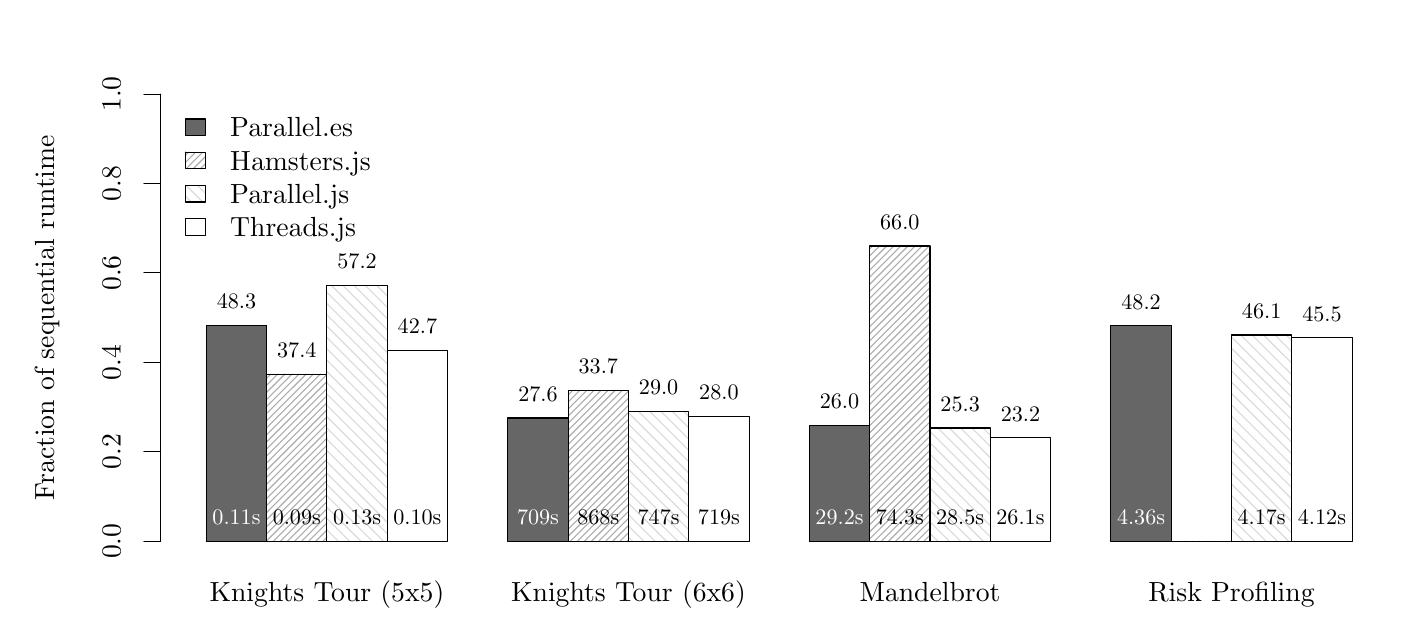
\begin{tikzpicture}[x=1pt,y=1pt]
\definecolor{fillColor}{RGB}{255,255,255}
\path[use as bounding box,fill=fillColor,fill opacity=0.00] (0,0) rectangle (495.15,209.58);
\begin{scope}
\path[clip] (  0.00,  0.00) rectangle (495.15,209.58);
\definecolor{fillColor}{gray}{0.40}

\path[fill=fillColor] ( 64.56, 24.00) --
	( 86.35, 24.00) --
	( 86.35,101.99) --
	( 64.56,101.99) --
	cycle;
\definecolor{drawColor}{RGB}{172,172,172}

\path[draw=drawColor,line width= 0.4pt,line join=round,line cap=round] ( 86.35, 82.91) -- ( 87.84, 84.40);

\path[draw=drawColor,line width= 0.4pt,line join=round,line cap=round] ( 86.35, 80.36) -- ( 90.40, 84.40);

\path[draw=drawColor,line width= 0.4pt,line join=round,line cap=round] ( 86.35, 77.80) -- ( 92.95, 84.40);

\path[draw=drawColor,line width= 0.4pt,line join=round,line cap=round] ( 86.35, 75.25) -- ( 95.51, 84.40);

\path[draw=drawColor,line width= 0.4pt,line join=round,line cap=round] ( 86.35, 72.69) -- ( 98.06, 84.40);

\path[draw=drawColor,line width= 0.4pt,line join=round,line cap=round] ( 86.35, 70.14) -- (100.62, 84.40);

\path[draw=drawColor,line width= 0.4pt,line join=round,line cap=round] ( 86.35, 67.58) -- (103.17, 84.40);

\path[draw=drawColor,line width= 0.4pt,line join=round,line cap=round] ( 86.35, 65.03) -- (105.73, 84.40);

\path[draw=drawColor,line width= 0.4pt,line join=round,line cap=round] ( 86.35, 62.47) -- (108.14, 84.26);

\path[draw=drawColor,line width= 0.4pt,line join=round,line cap=round] ( 86.35, 59.92) -- (108.14, 81.71);

\path[draw=drawColor,line width= 0.4pt,line join=round,line cap=round] ( 86.35, 57.36) -- (108.14, 79.15);

\path[draw=drawColor,line width= 0.4pt,line join=round,line cap=round] ( 86.35, 54.81) -- (108.14, 76.60);

\path[draw=drawColor,line width= 0.4pt,line join=round,line cap=round] ( 86.35, 52.25) -- (108.14, 74.04);

\path[draw=drawColor,line width= 0.4pt,line join=round,line cap=round] ( 86.35, 49.70) -- (108.14, 71.49);

\path[draw=drawColor,line width= 0.4pt,line join=round,line cap=round] ( 86.35, 47.14) -- (108.14, 68.93);

\path[draw=drawColor,line width= 0.4pt,line join=round,line cap=round] ( 86.35, 44.59) -- (108.14, 66.38);

\path[draw=drawColor,line width= 0.4pt,line join=round,line cap=round] ( 86.35, 42.03) -- (108.14, 63.82);

\path[draw=drawColor,line width= 0.4pt,line join=round,line cap=round] ( 86.35, 39.48) -- (108.14, 61.27);

\path[draw=drawColor,line width= 0.4pt,line join=round,line cap=round] ( 86.35, 36.92) -- (108.14, 58.71);

\path[draw=drawColor,line width= 0.4pt,line join=round,line cap=round] ( 86.35, 34.36) -- (108.14, 56.16);

\path[draw=drawColor,line width= 0.4pt,line join=round,line cap=round] ( 86.35, 31.81) -- (108.14, 53.60);

\path[draw=drawColor,line width= 0.4pt,line join=round,line cap=round] ( 86.35, 29.25) -- (108.14, 51.05);

\path[draw=drawColor,line width= 0.4pt,line join=round,line cap=round] ( 86.35, 26.70) -- (108.14, 48.49);

\path[draw=drawColor,line width= 0.4pt,line join=round,line cap=round] ( 86.35, 24.14) -- (108.14, 45.94);

\path[draw=drawColor,line width= 0.4pt,line join=round,line cap=round] ( 88.76, 24.00) -- (108.14, 43.38);

\path[draw=drawColor,line width= 0.4pt,line join=round,line cap=round] ( 91.32, 24.00) -- (108.14, 40.82);

\path[draw=drawColor,line width= 0.4pt,line join=round,line cap=round] ( 93.87, 24.00) -- (108.14, 38.27);

\path[draw=drawColor,line width= 0.4pt,line join=round,line cap=round] ( 96.43, 24.00) -- (108.14, 35.71);

\path[draw=drawColor,line width= 0.4pt,line join=round,line cap=round] ( 98.98, 24.00) -- (108.14, 33.16);

\path[draw=drawColor,line width= 0.4pt,line join=round,line cap=round] (101.54, 24.00) -- (108.14, 30.60);

\path[draw=drawColor,line width= 0.4pt,line join=round,line cap=round] (104.09, 24.00) -- (108.14, 28.05);

\path[draw=drawColor,line width= 0.4pt,line join=round,line cap=round] (106.65, 24.00) -- (108.14, 25.49);
\definecolor{drawColor}{RGB}{218,218,218}

\path[draw=drawColor,line width= 0.4pt,line join=round,line cap=round] (108.18, 24.00) -- (108.14, 24.04);

\path[draw=drawColor,line width= 0.4pt,line join=round,line cap=round] (112.27, 24.00) -- (108.14, 28.13);

\path[draw=drawColor,line width= 0.4pt,line join=round,line cap=round] (116.36, 24.00) -- (108.14, 32.22);

\path[draw=drawColor,line width= 0.4pt,line join=round,line cap=round] (120.45, 24.00) -- (108.14, 36.30);

\path[draw=drawColor,line width= 0.4pt,line join=round,line cap=round] (124.53, 24.00) -- (108.14, 40.39);

\path[draw=drawColor,line width= 0.4pt,line join=round,line cap=round] (128.62, 24.00) -- (108.14, 44.48);

\path[draw=drawColor,line width= 0.4pt,line join=round,line cap=round] (129.93, 26.78) -- (108.14, 48.57);

\path[draw=drawColor,line width= 0.4pt,line join=round,line cap=round] (129.93, 30.87) -- (108.14, 52.66);

\path[draw=drawColor,line width= 0.4pt,line join=round,line cap=round] (129.93, 34.95) -- (108.14, 56.74);

\path[draw=drawColor,line width= 0.4pt,line join=round,line cap=round] (129.93, 39.04) -- (108.14, 60.83);

\path[draw=drawColor,line width= 0.4pt,line join=round,line cap=round] (129.93, 43.13) -- (108.14, 64.92);

\path[draw=drawColor,line width= 0.4pt,line join=round,line cap=round] (129.93, 47.22) -- (108.14, 69.01);

\path[draw=drawColor,line width= 0.4pt,line join=round,line cap=round] (129.93, 51.31) -- (108.14, 73.10);

\path[draw=drawColor,line width= 0.4pt,line join=round,line cap=round] (129.93, 55.39) -- (108.14, 77.19);

\path[draw=drawColor,line width= 0.4pt,line join=round,line cap=round] (129.93, 59.48) -- (108.14, 81.27);

\path[draw=drawColor,line width= 0.4pt,line join=round,line cap=round] (129.93, 63.57) -- (108.14, 85.36);

\path[draw=drawColor,line width= 0.4pt,line join=round,line cap=round] (129.93, 67.66) -- (108.14, 89.45);

\path[draw=drawColor,line width= 0.4pt,line join=round,line cap=round] (129.93, 71.75) -- (108.14, 93.54);

\path[draw=drawColor,line width= 0.4pt,line join=round,line cap=round] (129.93, 75.84) -- (108.14, 97.63);

\path[draw=drawColor,line width= 0.4pt,line join=round,line cap=round] (129.93, 79.92) -- (108.14,101.71);

\path[draw=drawColor,line width= 0.4pt,line join=round,line cap=round] (129.93, 84.01) -- (108.14,105.80);

\path[draw=drawColor,line width= 0.4pt,line join=round,line cap=round] (129.93, 88.10) -- (108.14,109.89);

\path[draw=drawColor,line width= 0.4pt,line join=round,line cap=round] (129.93, 92.19) -- (108.14,113.98);

\path[draw=drawColor,line width= 0.4pt,line join=round,line cap=round] (129.93, 96.28) -- (109.81,116.40);

\path[draw=drawColor,line width= 0.4pt,line join=round,line cap=round] (129.93,100.37) -- (113.90,116.40);

\path[draw=drawColor,line width= 0.4pt,line join=round,line cap=round] (129.93,104.45) -- (117.98,116.40);

\path[draw=drawColor,line width= 0.4pt,line join=round,line cap=round] (129.93,108.54) -- (122.07,116.40);

\path[draw=drawColor,line width= 0.4pt,line join=round,line cap=round] (129.93,112.63) -- (126.16,116.40);

\path[fill=fillColor] (173.51, 24.00) --
	(195.31, 24.00) --
	(195.31, 68.53) --
	(173.51, 68.53) --
	cycle;
\definecolor{drawColor}{RGB}{172,172,172}

\path[draw=drawColor,line width= 0.4pt,line join=round,line cap=round] (195.31, 76.89) -- (196.93, 78.51);

\path[draw=drawColor,line width= 0.4pt,line join=round,line cap=round] (195.31, 74.33) -- (199.49, 78.51);

\path[draw=drawColor,line width= 0.4pt,line join=round,line cap=round] (195.31, 71.78) -- (202.04, 78.51);

\path[draw=drawColor,line width= 0.4pt,line join=round,line cap=round] (195.31, 69.22) -- (204.60, 78.51);

\path[draw=drawColor,line width= 0.4pt,line join=round,line cap=round] (195.31, 66.66) -- (207.15, 78.51);

\path[draw=drawColor,line width= 0.4pt,line join=round,line cap=round] (195.31, 64.11) -- (209.71, 78.51);

\path[draw=drawColor,line width= 0.4pt,line join=round,line cap=round] (195.31, 61.55) -- (212.26, 78.51);

\path[draw=drawColor,line width= 0.4pt,line join=round,line cap=round] (195.31, 59.00) -- (214.82, 78.51);

\path[draw=drawColor,line width= 0.4pt,line join=round,line cap=round] (195.31, 56.44) -- (217.10, 78.24);

\path[draw=drawColor,line width= 0.4pt,line join=round,line cap=round] (195.31, 53.89) -- (217.10, 75.68);

\path[draw=drawColor,line width= 0.4pt,line join=round,line cap=round] (195.31, 51.33) -- (217.10, 73.12);

\path[draw=drawColor,line width= 0.4pt,line join=round,line cap=round] (195.31, 48.78) -- (217.10, 70.57);

\path[draw=drawColor,line width= 0.4pt,line join=round,line cap=round] (195.31, 46.22) -- (217.10, 68.01);

\path[draw=drawColor,line width= 0.4pt,line join=round,line cap=round] (195.31, 43.67) -- (217.10, 65.46);

\path[draw=drawColor,line width= 0.4pt,line join=round,line cap=round] (195.31, 41.11) -- (217.10, 62.90);

\path[draw=drawColor,line width= 0.4pt,line join=round,line cap=round] (195.31, 38.56) -- (217.10, 60.35);

\path[draw=drawColor,line width= 0.4pt,line join=round,line cap=round] (195.31, 36.00) -- (217.10, 57.79);

\path[draw=drawColor,line width= 0.4pt,line join=round,line cap=round] (195.31, 33.45) -- (217.10, 55.24);

\path[draw=drawColor,line width= 0.4pt,line join=round,line cap=round] (195.31, 30.89) -- (217.10, 52.68);

\path[draw=drawColor,line width= 0.4pt,line join=round,line cap=round] (195.31, 28.34) -- (217.10, 50.13);

\path[draw=drawColor,line width= 0.4pt,line join=round,line cap=round] (195.31, 25.78) -- (217.10, 47.57);

\path[draw=drawColor,line width= 0.4pt,line join=round,line cap=round] (196.08, 24.00) -- (217.10, 45.02);

\path[draw=drawColor,line width= 0.4pt,line join=round,line cap=round] (198.63, 24.00) -- (217.10, 42.46);

\path[draw=drawColor,line width= 0.4pt,line join=round,line cap=round] (201.19, 24.00) -- (217.10, 39.91);

\path[draw=drawColor,line width= 0.4pt,line join=round,line cap=round] (203.74, 24.00) -- (217.10, 37.35);

\path[draw=drawColor,line width= 0.4pt,line join=round,line cap=round] (206.30, 24.00) -- (217.10, 34.80);

\path[draw=drawColor,line width= 0.4pt,line join=round,line cap=round] (208.85, 24.00) -- (217.10, 32.24);

\path[draw=drawColor,line width= 0.4pt,line join=round,line cap=round] (211.41, 24.00) -- (217.10, 29.69);

\path[draw=drawColor,line width= 0.4pt,line join=round,line cap=round] (213.96, 24.00) -- (217.10, 27.13);

\path[draw=drawColor,line width= 0.4pt,line join=round,line cap=round] (216.52, 24.00) -- (217.10, 24.58);
\definecolor{drawColor}{RGB}{218,218,218}

\path[draw=drawColor,line width= 0.4pt,line join=round,line cap=round] (218.56, 24.00) -- (217.10, 25.47);

\path[draw=drawColor,line width= 0.4pt,line join=round,line cap=round] (222.65, 24.00) -- (217.10, 29.55);

\path[draw=drawColor,line width= 0.4pt,line join=round,line cap=round] (226.74, 24.00) -- (217.10, 33.64);

\path[draw=drawColor,line width= 0.4pt,line join=round,line cap=round] (230.83, 24.00) -- (217.10, 37.73);

\path[draw=drawColor,line width= 0.4pt,line join=round,line cap=round] (234.92, 24.00) -- (217.10, 41.82);

\path[draw=drawColor,line width= 0.4pt,line join=round,line cap=round] (238.89, 24.12) -- (217.10, 45.91);

\path[draw=drawColor,line width= 0.4pt,line join=round,line cap=round] (238.89, 28.21) -- (217.10, 50.00);

\path[draw=drawColor,line width= 0.4pt,line join=round,line cap=round] (238.89, 32.29) -- (217.10, 54.08);

\path[draw=drawColor,line width= 0.4pt,line join=round,line cap=round] (238.89, 36.38) -- (217.10, 58.17);

\path[draw=drawColor,line width= 0.4pt,line join=round,line cap=round] (238.89, 40.47) -- (217.10, 62.26);

\path[draw=drawColor,line width= 0.4pt,line join=round,line cap=round] (238.89, 44.56) -- (217.10, 66.35);

\path[draw=drawColor,line width= 0.4pt,line join=round,line cap=round] (238.89, 48.65) -- (217.10, 70.44);

\path[draw=drawColor,line width= 0.4pt,line join=round,line cap=round] (238.89, 52.73) -- (220.75, 70.88);

\path[draw=drawColor,line width= 0.4pt,line join=round,line cap=round] (238.89, 56.82) -- (224.83, 70.88);

\path[draw=drawColor,line width= 0.4pt,line join=round,line cap=round] (238.89, 60.91) -- (228.92, 70.88);

\path[draw=drawColor,line width= 0.4pt,line join=round,line cap=round] (238.89, 65.00) -- (233.01, 70.88);

\path[draw=drawColor,line width= 0.4pt,line join=round,line cap=round] (238.89, 69.09) -- (237.10, 70.88);

\path[fill=fillColor] (282.47, 24.00) --
	(304.26, 24.00) --
	(304.26, 65.97) --
	(282.47, 65.97) --
	cycle;
\definecolor{drawColor}{RGB}{172,172,172}

\path[draw=drawColor,line width= 0.4pt,line join=round,line cap=round] (304.26,129.63) -- (305.33,130.70);

\path[draw=drawColor,line width= 0.4pt,line join=round,line cap=round] (304.26,127.07) -- (307.89,130.70);

\path[draw=drawColor,line width= 0.4pt,line join=round,line cap=round] (304.26,124.52) -- (310.44,130.70);

\path[draw=drawColor,line width= 0.4pt,line join=round,line cap=round] (304.26,121.96) -- (313.00,130.70);

\path[draw=drawColor,line width= 0.4pt,line join=round,line cap=round] (304.26,119.41) -- (315.55,130.70);

\path[draw=drawColor,line width= 0.4pt,line join=round,line cap=round] (304.26,116.85) -- (318.11,130.70);

\path[draw=drawColor,line width= 0.4pt,line join=round,line cap=round] (304.26,114.30) -- (320.67,130.70);

\path[draw=drawColor,line width= 0.4pt,line join=round,line cap=round] (304.26,111.74) -- (323.22,130.70);

\path[draw=drawColor,line width= 0.4pt,line join=round,line cap=round] (304.26,109.19) -- (325.78,130.70);

\path[draw=drawColor,line width= 0.4pt,line join=round,line cap=round] (304.26,106.63) -- (326.05,128.42);

\path[draw=drawColor,line width= 0.4pt,line join=round,line cap=round] (304.26,104.08) -- (326.05,125.87);

\path[draw=drawColor,line width= 0.4pt,line join=round,line cap=round] (304.26,101.52) -- (326.05,123.31);

\path[draw=drawColor,line width= 0.4pt,line join=round,line cap=round] (304.26, 98.96) -- (326.05,120.76);

\path[draw=drawColor,line width= 0.4pt,line join=round,line cap=round] (304.26, 96.41) -- (326.05,118.20);

\path[draw=drawColor,line width= 0.4pt,line join=round,line cap=round] (304.26, 93.85) -- (326.05,115.65);

\path[draw=drawColor,line width= 0.4pt,line join=round,line cap=round] (304.26, 91.30) -- (326.05,113.09);

\path[draw=drawColor,line width= 0.4pt,line join=round,line cap=round] (304.26, 88.74) -- (326.05,110.54);

\path[draw=drawColor,line width= 0.4pt,line join=round,line cap=round] (304.26, 86.19) -- (326.05,107.98);

\path[draw=drawColor,line width= 0.4pt,line join=round,line cap=round] (304.26, 83.63) -- (326.05,105.43);

\path[draw=drawColor,line width= 0.4pt,line join=round,line cap=round] (304.26, 81.08) -- (326.05,102.87);

\path[draw=drawColor,line width= 0.4pt,line join=round,line cap=round] (304.26, 78.52) -- (326.05,100.31);

\path[draw=drawColor,line width= 0.4pt,line join=round,line cap=round] (304.26, 75.97) -- (326.05, 97.76);

\path[draw=drawColor,line width= 0.4pt,line join=round,line cap=round] (304.26, 73.41) -- (326.05, 95.20);

\path[draw=drawColor,line width= 0.4pt,line join=round,line cap=round] (304.26, 70.86) -- (326.05, 92.65);

\path[draw=drawColor,line width= 0.4pt,line join=round,line cap=round] (304.26, 68.30) -- (326.05, 90.09);

\path[draw=drawColor,line width= 0.4pt,line join=round,line cap=round] (304.26, 65.75) -- (326.05, 87.54);

\path[draw=drawColor,line width= 0.4pt,line join=round,line cap=round] (304.26, 63.19) -- (326.05, 84.98);

\path[draw=drawColor,line width= 0.4pt,line join=round,line cap=round] (304.26, 60.64) -- (326.05, 82.43);

\path[draw=drawColor,line width= 0.4pt,line join=round,line cap=round] (304.26, 58.08) -- (326.05, 79.87);

\path[draw=drawColor,line width= 0.4pt,line join=round,line cap=round] (304.26, 55.53) -- (326.05, 77.32);

\path[draw=drawColor,line width= 0.4pt,line join=round,line cap=round] (304.26, 52.97) -- (326.05, 74.76);

\path[draw=drawColor,line width= 0.4pt,line join=round,line cap=round] (304.26, 50.42) -- (326.05, 72.21);

\path[draw=drawColor,line width= 0.4pt,line join=round,line cap=round] (304.26, 47.86) -- (326.05, 69.65);

\path[draw=drawColor,line width= 0.4pt,line join=round,line cap=round] (304.26, 45.31) -- (326.05, 67.10);

\path[draw=drawColor,line width= 0.4pt,line join=round,line cap=round] (304.26, 42.75) -- (326.05, 64.54);

\path[draw=drawColor,line width= 0.4pt,line join=round,line cap=round] (304.26, 40.20) -- (326.05, 61.99);

\path[draw=drawColor,line width= 0.4pt,line join=round,line cap=round] (304.26, 37.64) -- (326.05, 59.43);

\path[draw=drawColor,line width= 0.4pt,line join=round,line cap=round] (304.26, 35.09) -- (326.05, 56.88);

\path[draw=drawColor,line width= 0.4pt,line join=round,line cap=round] (304.26, 32.53) -- (326.05, 54.32);

\path[draw=drawColor,line width= 0.4pt,line join=round,line cap=round] (304.26, 29.98) -- (326.05, 51.77);

\path[draw=drawColor,line width= 0.4pt,line join=round,line cap=round] (304.26, 27.42) -- (326.05, 49.21);

\path[draw=drawColor,line width= 0.4pt,line join=round,line cap=round] (304.26, 24.87) -- (326.05, 46.66);

\path[draw=drawColor,line width= 0.4pt,line join=round,line cap=round] (305.95, 24.00) -- (326.05, 44.10);

\path[draw=drawColor,line width= 0.4pt,line join=round,line cap=round] (308.50, 24.00) -- (326.05, 41.55);

\path[draw=drawColor,line width= 0.4pt,line join=round,line cap=round] (311.06, 24.00) -- (326.05, 38.99);

\path[draw=drawColor,line width= 0.4pt,line join=round,line cap=round] (313.61, 24.00) -- (326.05, 36.44);

\path[draw=drawColor,line width= 0.4pt,line join=round,line cap=round] (316.17, 24.00) -- (326.05, 33.88);

\path[draw=drawColor,line width= 0.4pt,line join=round,line cap=round] (318.72, 24.00) -- (326.05, 31.33);

\path[draw=drawColor,line width= 0.4pt,line join=round,line cap=round] (321.28, 24.00) -- (326.05, 28.77);

\path[draw=drawColor,line width= 0.4pt,line join=round,line cap=round] (323.83, 24.00) -- (326.05, 26.22);
\definecolor{drawColor}{RGB}{218,218,218}

\path[draw=drawColor,line width= 0.4pt,line join=round,line cap=round] (328.94, 24.00) -- (326.05, 26.89);

\path[draw=drawColor,line width= 0.4pt,line join=round,line cap=round] (333.03, 24.00) -- (326.05, 30.98);

\path[draw=drawColor,line width= 0.4pt,line join=round,line cap=round] (337.12, 24.00) -- (326.05, 35.07);

\path[draw=drawColor,line width= 0.4pt,line join=round,line cap=round] (341.21, 24.00) -- (326.05, 39.16);

\path[draw=drawColor,line width= 0.4pt,line join=round,line cap=round] (345.30, 24.00) -- (326.05, 43.25);

\path[draw=drawColor,line width= 0.4pt,line join=round,line cap=round] (347.84, 25.54) -- (326.05, 47.34);

\path[draw=drawColor,line width= 0.4pt,line join=round,line cap=round] (347.84, 29.63) -- (326.05, 51.42);

\path[draw=drawColor,line width= 0.4pt,line join=round,line cap=round] (347.84, 33.72) -- (326.05, 55.51);

\path[draw=drawColor,line width= 0.4pt,line join=round,line cap=round] (347.84, 37.81) -- (326.05, 59.60);

\path[draw=drawColor,line width= 0.4pt,line join=round,line cap=round] (347.84, 41.90) -- (326.05, 63.69);

\path[draw=drawColor,line width= 0.4pt,line join=round,line cap=round] (347.84, 45.99) -- (328.90, 64.93);

\path[draw=drawColor,line width= 0.4pt,line join=round,line cap=round] (347.84, 50.07) -- (332.99, 64.93);

\path[draw=drawColor,line width= 0.4pt,line join=round,line cap=round] (347.84, 54.16) -- (337.08, 64.93);

\path[draw=drawColor,line width= 0.4pt,line join=round,line cap=round] (347.84, 58.25) -- (341.16, 64.93);

\path[draw=drawColor,line width= 0.4pt,line join=round,line cap=round] (347.84, 62.34) -- (345.25, 64.93);

\path[fill=fillColor] (391.42, 24.00) --
	(413.21, 24.00) --
	(413.21,101.88) --
	(391.42,101.88) --
	cycle;
\definecolor{drawColor}{RGB}{172,172,172}

\path[draw=drawColor,line width= 0.4pt,line join=round,line cap=round] (413.26, 24.00) -- (413.26, 24.00);

\path[draw=drawColor,line width= 0.4pt,line join=round,line cap=round] (415.82, 24.00) -- (415.82, 24.00);

\path[draw=drawColor,line width= 0.4pt,line join=round,line cap=round] (418.37, 24.00) -- (418.37, 24.00);

\path[draw=drawColor,line width= 0.4pt,line join=round,line cap=round] (420.93, 24.00) -- (420.93, 24.00);

\path[draw=drawColor,line width= 0.4pt,line join=round,line cap=round] (423.48, 24.00) -- (423.48, 24.00);

\path[draw=drawColor,line width= 0.4pt,line join=round,line cap=round] (426.04, 24.00) -- (426.04, 24.00);

\path[draw=drawColor,line width= 0.4pt,line join=round,line cap=round] (428.59, 24.00) -- (428.59, 24.00);

\path[draw=drawColor,line width= 0.4pt,line join=round,line cap=round] (431.15, 24.00) -- (431.15, 24.00);

\path[draw=drawColor,line width= 0.4pt,line join=round,line cap=round] (433.71, 24.00) -- (433.71, 24.00);
\definecolor{drawColor}{RGB}{218,218,218}

\path[draw=drawColor,line width= 0.4pt,line join=round,line cap=round] (435.24, 24.00) -- (435.00, 24.23);

\path[draw=drawColor,line width= 0.4pt,line join=round,line cap=round] (439.33, 24.00) -- (435.00, 28.32);

\path[draw=drawColor,line width= 0.4pt,line join=round,line cap=round] (443.41, 24.00) -- (435.00, 32.41);

\path[draw=drawColor,line width= 0.4pt,line join=round,line cap=round] (447.50, 24.00) -- (435.00, 36.50);

\path[draw=drawColor,line width= 0.4pt,line join=round,line cap=round] (451.59, 24.00) -- (435.00, 40.59);

\path[draw=drawColor,line width= 0.4pt,line join=round,line cap=round] (455.68, 24.00) -- (435.00, 44.67);

\path[draw=drawColor,line width= 0.4pt,line join=round,line cap=round] (456.80, 26.97) -- (435.00, 48.76);

\path[draw=drawColor,line width= 0.4pt,line join=round,line cap=round] (456.80, 31.06) -- (435.00, 52.85);

\path[draw=drawColor,line width= 0.4pt,line join=round,line cap=round] (456.80, 35.15) -- (435.00, 56.94);

\path[draw=drawColor,line width= 0.4pt,line join=round,line cap=round] (456.80, 39.24) -- (435.00, 61.03);

\path[draw=drawColor,line width= 0.4pt,line join=round,line cap=round] (456.80, 43.33) -- (435.00, 65.12);

\path[draw=drawColor,line width= 0.4pt,line join=round,line cap=round] (456.80, 47.41) -- (435.00, 69.20);

\path[draw=drawColor,line width= 0.4pt,line join=round,line cap=round] (456.80, 51.50) -- (435.00, 73.29);

\path[draw=drawColor,line width= 0.4pt,line join=round,line cap=round] (456.80, 55.59) -- (435.00, 77.38);

\path[draw=drawColor,line width= 0.4pt,line join=round,line cap=round] (456.80, 59.68) -- (435.00, 81.47);

\path[draw=drawColor,line width= 0.4pt,line join=round,line cap=round] (456.80, 63.77) -- (435.00, 85.56);

\path[draw=drawColor,line width= 0.4pt,line join=round,line cap=round] (456.80, 67.85) -- (435.00, 89.65);

\path[draw=drawColor,line width= 0.4pt,line join=round,line cap=round] (456.80, 71.94) -- (435.00, 93.73);

\path[draw=drawColor,line width= 0.4pt,line join=round,line cap=round] (456.80, 76.03) -- (435.00, 97.82);

\path[draw=drawColor,line width= 0.4pt,line join=round,line cap=round] (456.80, 80.12) -- (438.38, 98.53);

\path[draw=drawColor,line width= 0.4pt,line join=round,line cap=round] (456.80, 84.21) -- (442.47, 98.53);

\path[draw=drawColor,line width= 0.4pt,line join=round,line cap=round] (456.80, 88.30) -- (446.56, 98.53);

\path[draw=drawColor,line width= 0.4pt,line join=round,line cap=round] (456.80, 92.38) -- (450.65, 98.53);

\path[draw=drawColor,line width= 0.4pt,line join=round,line cap=round] (456.80, 96.47) -- (454.73, 98.53);
\definecolor{drawColor}{RGB}{0,0,0}

\path[draw=drawColor,line width= 0.4pt,line join=round,line cap=round] ( 64.56, 24.00) --
	( 86.35, 24.00) --
	( 86.35,101.99) --
	( 64.56,101.99) --
	( 64.56, 24.00);

\path[draw=drawColor,line width= 0.4pt,line join=round,line cap=round] ( 86.35, 24.00) --
	(108.14, 24.00) --
	(108.14, 84.40) --
	( 86.35, 84.40) --
	( 86.35, 24.00);

\path[draw=drawColor,line width= 0.4pt,line join=round,line cap=round] (108.14, 24.00) --
	(129.93, 24.00) --
	(129.93,116.40) --
	(108.14,116.40) --
	(108.14, 24.00);

\path[draw=drawColor,line width= 0.4pt,line join=round,line cap=round] (129.93, 24.00) --
	(151.72, 24.00) --
	(151.72, 93.01) --
	(129.93, 93.01) --
	(129.93, 24.00);

\path[draw=drawColor,line width= 0.4pt,line join=round,line cap=round] (173.51, 24.00) --
	(195.31, 24.00) --
	(195.31, 68.53) --
	(173.51, 68.53) --
	(173.51, 24.00);

\path[draw=drawColor,line width= 0.4pt,line join=round,line cap=round] (195.31, 24.00) --
	(217.10, 24.00) --
	(217.10, 78.51) --
	(195.31, 78.51) --
	(195.31, 24.00);

\path[draw=drawColor,line width= 0.4pt,line join=round,line cap=round] (217.10, 24.00) --
	(238.89, 24.00) --
	(238.89, 70.88) --
	(217.10, 70.88) --
	(217.10, 24.00);

\path[draw=drawColor,line width= 0.4pt,line join=round,line cap=round] (238.89, 24.00) --
	(260.68, 24.00) --
	(260.68, 69.17) --
	(238.89, 69.17) --
	(238.89, 24.00);

\path[draw=drawColor,line width= 0.4pt,line join=round,line cap=round] (282.47, 24.00) --
	(304.26, 24.00) --
	(304.26, 65.97) --
	(282.47, 65.97) --
	(282.47, 24.00);

\path[draw=drawColor,line width= 0.4pt,line join=round,line cap=round] (304.26, 24.00) --
	(326.05, 24.00) --
	(326.05,130.70) --
	(304.26,130.70) --
	(304.26, 24.00);

\path[draw=drawColor,line width= 0.4pt,line join=round,line cap=round] (326.05, 24.00) --
	(347.84, 24.00) --
	(347.84, 64.93) --
	(326.05, 64.93) --
	(326.05, 24.00);

\path[draw=drawColor,line width= 0.4pt,line join=round,line cap=round] (347.84, 24.00) --
	(369.63, 24.00) --
	(369.63, 61.41) --
	(347.84, 61.41) --
	(347.84, 24.00);

\path[draw=drawColor,line width= 0.4pt,line join=round,line cap=round] (391.42, 24.00) --
	(413.21, 24.00) --
	(413.21,101.88) --
	(391.42,101.88) --
	(391.42, 24.00);

\path[draw=drawColor,line width= 0.4pt,line join=round,line cap=round] (413.21, 24.00) --
	(435.00, 24.00) --
	(413.21, 24.00);

\path[draw=drawColor,line width= 0.4pt,line join=round,line cap=round] (435.00, 24.00) --
	(456.80, 24.00) --
	(456.80, 98.53) --
	(435.00, 98.53) --
	(435.00, 24.00);

\path[draw=drawColor,line width= 0.4pt,line join=round,line cap=round] (456.80, 24.00) --
	(478.59, 24.00) --
	(478.59, 97.58) --
	(456.80, 97.58) --
	(456.80, 24.00);
\end{scope}
\begin{scope}
\path[clip] (  0.00,  0.00) rectangle (495.15,209.58);
\definecolor{drawColor}{RGB}{0,0,0}

\node[text=drawColor,anchor=base,inner sep=0pt, outer sep=0pt, scale=  1.00] at (108.14,  2.40) {Knights Tour (5x5)};

\node[text=drawColor,anchor=base,inner sep=0pt, outer sep=0pt, scale=  1.00] at (217.10,  2.40) {Knights Tour (6x6)};

\node[text=drawColor,anchor=base,inner sep=0pt, outer sep=0pt, scale=  1.00] at (326.05,  2.40) {Mandelbrot};

\node[text=drawColor,anchor=base,inner sep=0pt, outer sep=0pt, scale=  1.00] at (435.00,  2.40) {Risk Profiling};
\end{scope}
\begin{scope}
\path[clip] (  0.00,  0.00) rectangle (495.15,209.58);
\definecolor{drawColor}{RGB}{0,0,0}

\node[text=drawColor,rotate= 90.00,anchor=base,inner sep=0pt, outer sep=0pt, scale=  1.00] at (  9.60,104.79) {Fraction of sequential runtime};
\end{scope}
\begin{scope}
\path[clip] (  0.00,  0.00) rectangle (495.15,209.58);
\definecolor{drawColor}{RGB}{0,0,0}

\path[draw=drawColor,line width= 0.4pt,line join=round,line cap=round] ( 48.00, 24.00) -- ( 48.00,185.58);

\path[draw=drawColor,line width= 0.4pt,line join=round,line cap=round] ( 48.00, 24.00) -- ( 42.00, 24.00);

\path[draw=drawColor,line width= 0.4pt,line join=round,line cap=round] ( 48.00, 56.32) -- ( 42.00, 56.32);

\path[draw=drawColor,line width= 0.4pt,line join=round,line cap=round] ( 48.00, 88.63) -- ( 42.00, 88.63);

\path[draw=drawColor,line width= 0.4pt,line join=round,line cap=round] ( 48.00,120.95) -- ( 42.00,120.95);

\path[draw=drawColor,line width= 0.4pt,line join=round,line cap=round] ( 48.00,153.27) -- ( 42.00,153.27);

\path[draw=drawColor,line width= 0.4pt,line join=round,line cap=round] ( 48.00,185.58) -- ( 42.00,185.58);

\node[text=drawColor,rotate= 90.00,anchor=base,inner sep=0pt, outer sep=0pt, scale=  1.00] at ( 33.60, 24.00) {0.0};

\node[text=drawColor,rotate= 90.00,anchor=base,inner sep=0pt, outer sep=0pt, scale=  1.00] at ( 33.60, 56.32) {0.2};

\node[text=drawColor,rotate= 90.00,anchor=base,inner sep=0pt, outer sep=0pt, scale=  1.00] at ( 33.60, 88.63) {0.4};

\node[text=drawColor,rotate= 90.00,anchor=base,inner sep=0pt, outer sep=0pt, scale=  1.00] at ( 33.60,120.95) {0.6};

\node[text=drawColor,rotate= 90.00,anchor=base,inner sep=0pt, outer sep=0pt, scale=  1.00] at ( 33.60,153.27) {0.8};

\node[text=drawColor,rotate= 90.00,anchor=base,inner sep=0pt, outer sep=0pt, scale=  1.00] at ( 33.60,185.58) {1.0};
\end{scope}
\begin{scope}
\path[clip] ( 48.00, 24.00) rectangle (495.15,185.58);
\definecolor{fillColor}{gray}{0.40}

\path[fill=fillColor] ( 57.00,176.58) --
	( 64.20,176.58) --
	( 64.20,170.58) --
	( 57.00,170.58) --
	cycle;
\definecolor{drawColor}{RGB}{172,172,172}

\path[draw=drawColor,line width= 0.4pt,line join=round,line cap=round] ( 57.00,163.43) -- ( 58.15,164.58);

\path[draw=drawColor,line width= 0.4pt,line join=round,line cap=round] ( 57.00,160.88) -- ( 60.71,164.58);

\path[draw=drawColor,line width= 0.4pt,line join=round,line cap=round] ( 57.26,158.58) -- ( 63.26,164.58);

\path[draw=drawColor,line width= 0.4pt,line join=round,line cap=round] ( 59.82,158.58) -- ( 64.20,162.97);

\path[draw=drawColor,line width= 0.4pt,line join=round,line cap=round] ( 62.37,158.58) -- ( 64.20,160.41);
\definecolor{drawColor}{RGB}{218,218,218}

\path[draw=drawColor,line width= 0.4pt,line join=round,line cap=round] ( 59.19,146.58) -- ( 57.00,148.77);

\path[draw=drawColor,line width= 0.4pt,line join=round,line cap=round] ( 63.27,146.58) -- ( 57.27,152.58);

\path[draw=drawColor,line width= 0.4pt,line join=round,line cap=round] ( 64.20,149.75) -- ( 61.36,152.58);
\definecolor{drawColor}{RGB}{0,0,0}

\path[draw=drawColor,line width= 0.4pt,line join=round,line cap=round] ( 57.00,176.58) --
	( 64.20,176.58) --
	( 64.20,170.58) --
	( 57.00,170.58) --
	( 57.00,176.58);

\path[draw=drawColor,line width= 0.4pt,line join=round,line cap=round] ( 57.00,164.58) --
	( 64.20,164.58) --
	( 64.20,158.58) --
	( 57.00,158.58) --
	( 57.00,164.58);

\path[draw=drawColor,line width= 0.4pt,line join=round,line cap=round] ( 57.00,152.58) --
	( 64.20,152.58) --
	( 64.20,146.58) --
	( 57.00,146.58) --
	( 57.00,152.58);

\path[draw=drawColor,line width= 0.4pt,line join=round,line cap=round] ( 57.00,140.58) --
	( 64.20,140.58) --
	( 64.20,134.58) --
	( 57.00,134.58) --
	( 57.00,140.58);

\node[text=drawColor,anchor=base west,inner sep=0pt, outer sep=0pt, scale=  1.00] at ( 73.20,170.14) {Parallel.es};

\node[text=drawColor,anchor=base west,inner sep=0pt, outer sep=0pt, scale=  1.00] at ( 73.20,158.14) {Hamsters.js};

\node[text=drawColor,anchor=base west,inner sep=0pt, outer sep=0pt, scale=  1.00] at ( 73.20,146.14) {Parallel.js};

\node[text=drawColor,anchor=base west,inner sep=0pt, outer sep=0pt, scale=  1.00] at ( 73.20,134.14) {Threads.js};

\node[text=drawColor,anchor=base,inner sep=0pt, outer sep=0pt, scale=  0.80] at ( 75.46,107.99) {48.3};

\node[text=drawColor,anchor=base,inner sep=0pt, outer sep=0pt, scale=  0.80] at ( 97.25, 90.40) {37.4};

\node[text=drawColor,anchor=base,inner sep=0pt, outer sep=0pt, scale=  0.80] at (119.04,122.40) {57.2};

\node[text=drawColor,anchor=base,inner sep=0pt, outer sep=0pt, scale=  0.80] at (140.83, 99.01) {42.7};

\node[text=drawColor,anchor=base,inner sep=0pt, outer sep=0pt, scale=  0.80] at (184.41, 74.53) {27.6};

\node[text=drawColor,anchor=base,inner sep=0pt, outer sep=0pt, scale=  0.80] at (206.20, 84.51) {33.7};

\node[text=drawColor,anchor=base,inner sep=0pt, outer sep=0pt, scale=  0.80] at (227.99, 76.88) {29.0};

\node[text=drawColor,anchor=base,inner sep=0pt, outer sep=0pt, scale=  0.80] at (249.78, 75.17) {28.0};

\node[text=drawColor,anchor=base,inner sep=0pt, outer sep=0pt, scale=  0.80] at (293.36, 71.97) {26.0};

\node[text=drawColor,anchor=base,inner sep=0pt, outer sep=0pt, scale=  0.80] at (315.16,136.70) {66.0};

\node[text=drawColor,anchor=base,inner sep=0pt, outer sep=0pt, scale=  0.80] at (336.95, 70.93) {25.3};

\node[text=drawColor,anchor=base,inner sep=0pt, outer sep=0pt, scale=  0.80] at (358.74, 67.41) {23.2};

\node[text=drawColor,anchor=base,inner sep=0pt, outer sep=0pt, scale=  0.80] at (402.32,107.88) {48.2};

\node[text=drawColor,anchor=base,inner sep=0pt, outer sep=0pt, scale=  0.80] at (445.90,104.53) {46.1};

\node[text=drawColor,anchor=base,inner sep=0pt, outer sep=0pt, scale=  0.80] at (467.69,103.58) {45.5};
\definecolor{drawColor}{RGB}{255,255,255}

\node[text=drawColor,anchor=base,inner sep=0pt, outer sep=0pt, scale=  0.80] at ( 75.46, 30.00) {0.11s};
\definecolor{drawColor}{RGB}{0,0,0}

\node[text=drawColor,anchor=base,inner sep=0pt, outer sep=0pt, scale=  0.80] at ( 97.25, 30.00) {0.09s};

\node[text=drawColor,anchor=base,inner sep=0pt, outer sep=0pt, scale=  0.80] at (119.04, 30.00) {0.13s};

\node[text=drawColor,anchor=base,inner sep=0pt, outer sep=0pt, scale=  0.80] at (140.83, 30.00) {0.10s};
\definecolor{drawColor}{RGB}{255,255,255}

\node[text=drawColor,anchor=base,inner sep=0pt, outer sep=0pt, scale=  0.80] at (184.41, 30.00) {709s};
\definecolor{drawColor}{RGB}{0,0,0}

\node[text=drawColor,anchor=base,inner sep=0pt, outer sep=0pt, scale=  0.80] at (206.20, 30.00) {868s};

\node[text=drawColor,anchor=base,inner sep=0pt, outer sep=0pt, scale=  0.80] at (227.99, 30.00) {747s};

\node[text=drawColor,anchor=base,inner sep=0pt, outer sep=0pt, scale=  0.80] at (249.78, 30.00) {719s};
\definecolor{drawColor}{RGB}{255,255,255}

\node[text=drawColor,anchor=base,inner sep=0pt, outer sep=0pt, scale=  0.80] at (293.36, 30.00) {29.2s};
\definecolor{drawColor}{RGB}{0,0,0}

\node[text=drawColor,anchor=base,inner sep=0pt, outer sep=0pt, scale=  0.80] at (315.16, 30.00) {74.3s};

\node[text=drawColor,anchor=base,inner sep=0pt, outer sep=0pt, scale=  0.80] at (336.95, 30.00) {28.5s};

\node[text=drawColor,anchor=base,inner sep=0pt, outer sep=0pt, scale=  0.80] at (358.74, 30.00) {26.1s};
\definecolor{drawColor}{RGB}{255,255,255}

\node[text=drawColor,anchor=base,inner sep=0pt, outer sep=0pt, scale=  0.80] at (402.32, 30.00) {4.36s};
\definecolor{drawColor}{RGB}{0,0,0}

\node[text=drawColor,anchor=base,inner sep=0pt, outer sep=0pt, scale=  0.80] at (445.90, 30.00) {4.17s};

\node[text=drawColor,anchor=base,inner sep=0pt, outer sep=0pt, scale=  0.80] at (467.69, 30.00) {4.12s};
\end{scope}
\end{tikzpicture}
	
	\caption{Runtime Performance of Parallelization Problems Relative to Synchronous Execution}
	\label{fig:runtime-performance}
\end{figure*}


\paragraph{Knight Tour} The time needed to solve the knight tour problem is mainly determined by the available computational resources. The calculation is parallelized by computing the number of tours starting from a specific start-field sequence and summarizing the number of found tours at the end. 

Parallel.js creates new tasks for accumulating the sub-results of start-field sequences computed by two tasks and executes them on designated background threads. That results in a significant overhead for the smaller $5\times5$ board. However, the impact is no longer visible for the larger board.

The results of Firefox do not indicate that using a thread pool to avoid spawning new background threads for every task is beneficial. It seems that creating background threads in Firefox is very inexpensive. However, the benchmarking results of Google Chrome shown in \cref{fig:runtime-performance-chrome} give evidence that a thread pool might be advantageous for very short running tasks. Thus, Hamsters.js and Parallel.es achieve slightly better results than Parallel.js, that is not using a thread pool at all, and Threads.js, where a new thread pool is created manually for each execution\footnote{A new thread pool for each run is not strictly necessary for the knight tour problem. However, it is needed to store the simulation result of the risk profiling problem.}. 

\begin{figure}
	\centering
	% Created by tikzDevice version 0.10.1 on 2016-12-09 07:37:51
% !TEX encoding = UTF-8 Unicode
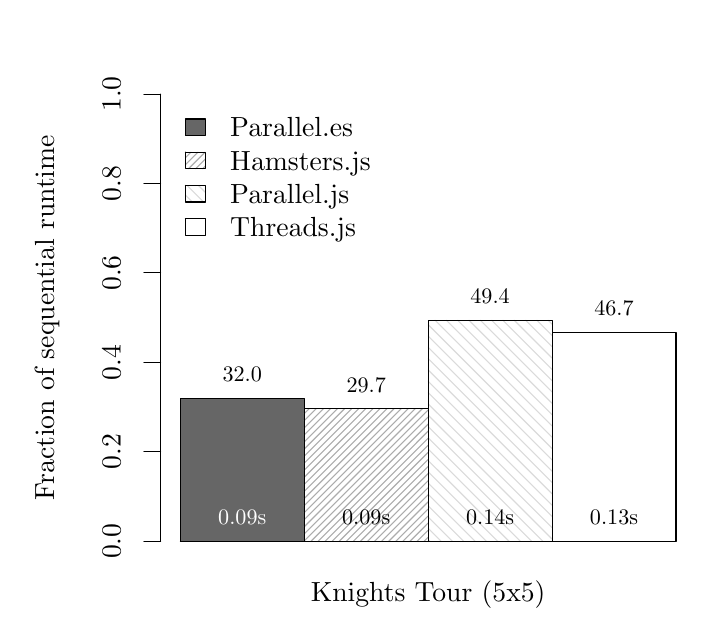
\begin{tikzpicture}[x=1pt,y=1pt]
\definecolor{fillColor}{RGB}{255,255,255}
\path[use as bounding box,fill=fillColor,fill opacity=0.00] (0,0) rectangle (241.43,209.58);
\begin{scope}
\path[clip] (  0.00,  0.00) rectangle (241.43,209.58);
\definecolor{fillColor}{gray}{0.40}

\path[fill=fillColor] ( 55.16, 24.00) --
	( 99.94, 24.00) --
	( 99.94, 75.63) --
	( 55.16, 75.63) --
	cycle;
\definecolor{drawColor}{RGB}{172,172,172}

\path[draw=drawColor,line width= 0.4pt,line join=round,line cap=round] ( 99.94, 70.11) -- (101.74, 71.91);

\path[draw=drawColor,line width= 0.4pt,line join=round,line cap=round] ( 99.94, 67.56) -- (104.29, 71.91);

\path[draw=drawColor,line width= 0.4pt,line join=round,line cap=round] ( 99.94, 65.00) -- (106.85, 71.91);

\path[draw=drawColor,line width= 0.4pt,line join=round,line cap=round] ( 99.94, 62.45) -- (109.40, 71.91);

\path[draw=drawColor,line width= 0.4pt,line join=round,line cap=round] ( 99.94, 59.89) -- (111.96, 71.91);

\path[draw=drawColor,line width= 0.4pt,line join=round,line cap=round] ( 99.94, 57.34) -- (114.51, 71.91);

\path[draw=drawColor,line width= 0.4pt,line join=round,line cap=round] ( 99.94, 54.78) -- (117.07, 71.91);

\path[draw=drawColor,line width= 0.4pt,line join=round,line cap=round] ( 99.94, 52.23) -- (119.62, 71.91);

\path[draw=drawColor,line width= 0.4pt,line join=round,line cap=round] ( 99.94, 49.67) -- (122.18, 71.91);

\path[draw=drawColor,line width= 0.4pt,line join=round,line cap=round] ( 99.94, 47.12) -- (124.74, 71.91);

\path[draw=drawColor,line width= 0.4pt,line join=round,line cap=round] ( 99.94, 44.56) -- (127.29, 71.91);

\path[draw=drawColor,line width= 0.4pt,line join=round,line cap=round] ( 99.94, 42.01) -- (129.85, 71.91);

\path[draw=drawColor,line width= 0.4pt,line join=round,line cap=round] ( 99.94, 39.45) -- (132.40, 71.91);

\path[draw=drawColor,line width= 0.4pt,line join=round,line cap=round] ( 99.94, 36.90) -- (134.96, 71.91);

\path[draw=drawColor,line width= 0.4pt,line join=round,line cap=round] ( 99.94, 34.34) -- (137.51, 71.91);

\path[draw=drawColor,line width= 0.4pt,line join=round,line cap=round] ( 99.94, 31.79) -- (140.07, 71.91);

\path[draw=drawColor,line width= 0.4pt,line join=round,line cap=round] ( 99.94, 29.23) -- (142.62, 71.91);

\path[draw=drawColor,line width= 0.4pt,line join=round,line cap=round] ( 99.94, 26.68) -- (144.71, 71.45);

\path[draw=drawColor,line width= 0.4pt,line join=round,line cap=round] ( 99.94, 24.12) -- (144.71, 68.90);

\path[draw=drawColor,line width= 0.4pt,line join=round,line cap=round] (102.37, 24.00) -- (144.71, 66.34);

\path[draw=drawColor,line width= 0.4pt,line join=round,line cap=round] (104.93, 24.00) -- (144.71, 63.79);

\path[draw=drawColor,line width= 0.4pt,line join=round,line cap=round] (107.48, 24.00) -- (144.71, 61.23);

\path[draw=drawColor,line width= 0.4pt,line join=round,line cap=round] (110.04, 24.00) -- (144.71, 58.68);

\path[draw=drawColor,line width= 0.4pt,line join=round,line cap=round] (112.59, 24.00) -- (144.71, 56.12);

\path[draw=drawColor,line width= 0.4pt,line join=round,line cap=round] (115.15, 24.00) -- (144.71, 53.57);

\path[draw=drawColor,line width= 0.4pt,line join=round,line cap=round] (117.70, 24.00) -- (144.71, 51.01);

\path[draw=drawColor,line width= 0.4pt,line join=round,line cap=round] (120.26, 24.00) -- (144.71, 48.45);

\path[draw=drawColor,line width= 0.4pt,line join=round,line cap=round] (122.81, 24.00) -- (144.71, 45.90);

\path[draw=drawColor,line width= 0.4pt,line join=round,line cap=round] (125.37, 24.00) -- (144.71, 43.34);

\path[draw=drawColor,line width= 0.4pt,line join=round,line cap=round] (127.92, 24.00) -- (144.71, 40.79);

\path[draw=drawColor,line width= 0.4pt,line join=round,line cap=round] (130.48, 24.00) -- (144.71, 38.23);

\path[draw=drawColor,line width= 0.4pt,line join=round,line cap=round] (133.04, 24.00) -- (144.71, 35.68);

\path[draw=drawColor,line width= 0.4pt,line join=round,line cap=round] (135.59, 24.00) -- (144.71, 33.12);

\path[draw=drawColor,line width= 0.4pt,line join=round,line cap=round] (138.15, 24.00) -- (144.71, 30.57);

\path[draw=drawColor,line width= 0.4pt,line join=round,line cap=round] (140.70, 24.00) -- (144.71, 28.01);

\path[draw=drawColor,line width= 0.4pt,line join=round,line cap=round] (143.26, 24.00) -- (144.71, 25.46);
\definecolor{drawColor}{RGB}{218,218,218}

\path[draw=drawColor,line width= 0.4pt,line join=round,line cap=round] (145.30, 24.00) -- (144.71, 24.59);

\path[draw=drawColor,line width= 0.4pt,line join=round,line cap=round] (149.39, 24.00) -- (144.71, 28.67);

\path[draw=drawColor,line width= 0.4pt,line join=round,line cap=round] (153.48, 24.00) -- (144.71, 32.76);

\path[draw=drawColor,line width= 0.4pt,line join=round,line cap=round] (157.56, 24.00) -- (144.71, 36.85);

\path[draw=drawColor,line width= 0.4pt,line join=round,line cap=round] (161.65, 24.00) -- (144.71, 40.94);

\path[draw=drawColor,line width= 0.4pt,line join=round,line cap=round] (165.74, 24.00) -- (144.71, 45.03);

\path[draw=drawColor,line width= 0.4pt,line join=round,line cap=round] (169.83, 24.00) -- (144.71, 49.11);

\path[draw=drawColor,line width= 0.4pt,line join=round,line cap=round] (173.92, 24.00) -- (144.71, 53.20);

\path[draw=drawColor,line width= 0.4pt,line join=round,line cap=round] (178.01, 24.00) -- (144.71, 57.29);

\path[draw=drawColor,line width= 0.4pt,line join=round,line cap=round] (182.09, 24.00) -- (144.71, 61.38);

\path[draw=drawColor,line width= 0.4pt,line join=round,line cap=round] (186.18, 24.00) -- (144.71, 65.47);

\path[draw=drawColor,line width= 0.4pt,line join=round,line cap=round] (189.49, 24.78) -- (144.71, 69.56);

\path[draw=drawColor,line width= 0.4pt,line join=round,line cap=round] (189.49, 28.87) -- (144.71, 73.64);

\path[draw=drawColor,line width= 0.4pt,line join=round,line cap=round] (189.49, 32.96) -- (144.71, 77.73);

\path[draw=drawColor,line width= 0.4pt,line join=round,line cap=round] (189.49, 37.05) -- (144.71, 81.82);

\path[draw=drawColor,line width= 0.4pt,line join=round,line cap=round] (189.49, 41.13) -- (144.71, 85.91);

\path[draw=drawColor,line width= 0.4pt,line join=round,line cap=round] (189.49, 45.22) -- (144.71, 90.00);

\path[draw=drawColor,line width= 0.4pt,line join=round,line cap=round] (189.49, 49.31) -- (144.71, 94.08);

\path[draw=drawColor,line width= 0.4pt,line join=round,line cap=round] (189.49, 53.40) -- (144.71, 98.17);

\path[draw=drawColor,line width= 0.4pt,line join=round,line cap=round] (189.49, 57.49) -- (144.71,102.26);

\path[draw=drawColor,line width= 0.4pt,line join=round,line cap=round] (189.49, 61.57) -- (147.23,103.83);

\path[draw=drawColor,line width= 0.4pt,line join=round,line cap=round] (189.49, 65.66) -- (151.32,103.83);

\path[draw=drawColor,line width= 0.4pt,line join=round,line cap=round] (189.49, 69.75) -- (155.41,103.83);

\path[draw=drawColor,line width= 0.4pt,line join=round,line cap=round] (189.49, 73.84) -- (159.50,103.83);

\path[draw=drawColor,line width= 0.4pt,line join=round,line cap=round] (189.49, 77.93) -- (163.59,103.83);

\path[draw=drawColor,line width= 0.4pt,line join=round,line cap=round] (189.49, 82.02) -- (167.67,103.83);

\path[draw=drawColor,line width= 0.4pt,line join=round,line cap=round] (189.49, 86.10) -- (171.76,103.83);

\path[draw=drawColor,line width= 0.4pt,line join=round,line cap=round] (189.49, 90.19) -- (175.85,103.83);

\path[draw=drawColor,line width= 0.4pt,line join=round,line cap=round] (189.49, 94.28) -- (179.94,103.83);

\path[draw=drawColor,line width= 0.4pt,line join=round,line cap=round] (189.49, 98.37) -- (184.03,103.83);

\path[draw=drawColor,line width= 0.4pt,line join=round,line cap=round] (189.49,102.46) -- (188.12,103.83);
\definecolor{drawColor}{RGB}{0,0,0}

\path[draw=drawColor,line width= 0.4pt,line join=round,line cap=round] ( 55.16, 24.00) --
	( 99.94, 24.00) --
	( 99.94, 75.63) --
	( 55.16, 75.63) --
	( 55.16, 24.00);

\path[draw=drawColor,line width= 0.4pt,line join=round,line cap=round] ( 99.94, 24.00) --
	(144.71, 24.00) --
	(144.71, 71.91) --
	( 99.94, 71.91) --
	( 99.94, 24.00);

\path[draw=drawColor,line width= 0.4pt,line join=round,line cap=round] (144.71, 24.00) --
	(189.49, 24.00) --
	(189.49,103.83) --
	(144.71,103.83) --
	(144.71, 24.00);

\path[draw=drawColor,line width= 0.4pt,line join=round,line cap=round] (189.49, 24.00) --
	(234.26, 24.00) --
	(234.26, 99.46) --
	(189.49, 99.46) --
	(189.49, 24.00);
\end{scope}
\begin{scope}
\path[clip] (  0.00,  0.00) rectangle (241.43,209.58);
\definecolor{drawColor}{RGB}{0,0,0}

\node[text=drawColor,anchor=base,inner sep=0pt, outer sep=0pt, scale=  1.00] at (144.71,  2.40) {Knights Tour (5x5)};
\end{scope}
\begin{scope}
\path[clip] (  0.00,  0.00) rectangle (241.43,209.58);
\definecolor{drawColor}{RGB}{0,0,0}

\node[text=drawColor,rotate= 90.00,anchor=base,inner sep=0pt, outer sep=0pt, scale=  1.00] at (  9.60,104.79) {Fraction of sequential runtime};
\end{scope}
\begin{scope}
\path[clip] (  0.00,  0.00) rectangle (241.43,209.58);
\definecolor{drawColor}{RGB}{0,0,0}

\path[draw=drawColor,line width= 0.4pt,line join=round,line cap=round] ( 48.00, 24.00) -- ( 48.00,185.58);

\path[draw=drawColor,line width= 0.4pt,line join=round,line cap=round] ( 48.00, 24.00) -- ( 42.00, 24.00);

\path[draw=drawColor,line width= 0.4pt,line join=round,line cap=round] ( 48.00, 56.32) -- ( 42.00, 56.32);

\path[draw=drawColor,line width= 0.4pt,line join=round,line cap=round] ( 48.00, 88.63) -- ( 42.00, 88.63);

\path[draw=drawColor,line width= 0.4pt,line join=round,line cap=round] ( 48.00,120.95) -- ( 42.00,120.95);

\path[draw=drawColor,line width= 0.4pt,line join=round,line cap=round] ( 48.00,153.27) -- ( 42.00,153.27);

\path[draw=drawColor,line width= 0.4pt,line join=round,line cap=round] ( 48.00,185.58) -- ( 42.00,185.58);

\node[text=drawColor,rotate= 90.00,anchor=base,inner sep=0pt, outer sep=0pt, scale=  1.00] at ( 33.60, 24.00) {0.0};

\node[text=drawColor,rotate= 90.00,anchor=base,inner sep=0pt, outer sep=0pt, scale=  1.00] at ( 33.60, 56.32) {0.2};

\node[text=drawColor,rotate= 90.00,anchor=base,inner sep=0pt, outer sep=0pt, scale=  1.00] at ( 33.60, 88.63) {0.4};

\node[text=drawColor,rotate= 90.00,anchor=base,inner sep=0pt, outer sep=0pt, scale=  1.00] at ( 33.60,120.95) {0.6};

\node[text=drawColor,rotate= 90.00,anchor=base,inner sep=0pt, outer sep=0pt, scale=  1.00] at ( 33.60,153.27) {0.8};

\node[text=drawColor,rotate= 90.00,anchor=base,inner sep=0pt, outer sep=0pt, scale=  1.00] at ( 33.60,185.58) {1.0};
\end{scope}
\begin{scope}
\path[clip] ( 48.00, 24.00) rectangle (241.43,185.58);
\definecolor{fillColor}{gray}{0.40}

\path[fill=fillColor] ( 57.00,176.58) --
	( 64.20,176.58) --
	( 64.20,170.58) --
	( 57.00,170.58) --
	cycle;
\definecolor{drawColor}{RGB}{172,172,172}

\path[draw=drawColor,line width= 0.4pt,line join=round,line cap=round] ( 57.00,162.60) -- ( 58.99,164.58);

\path[draw=drawColor,line width= 0.4pt,line join=round,line cap=round] ( 57.00,160.04) -- ( 61.54,164.58);

\path[draw=drawColor,line width= 0.4pt,line join=round,line cap=round] ( 58.10,158.58) -- ( 64.10,164.58);

\path[draw=drawColor,line width= 0.4pt,line join=round,line cap=round] ( 60.65,158.58) -- ( 64.20,162.13);

\path[draw=drawColor,line width= 0.4pt,line join=round,line cap=round] ( 63.21,158.58) -- ( 64.20,159.58);
\definecolor{drawColor}{RGB}{218,218,218}

\path[draw=drawColor,line width= 0.4pt,line join=round,line cap=round] ( 59.51,146.58) -- ( 57.00,149.09);

\path[draw=drawColor,line width= 0.4pt,line join=round,line cap=round] ( 63.60,146.58) -- ( 57.60,152.58);

\path[draw=drawColor,line width= 0.4pt,line join=round,line cap=round] ( 64.20,150.07) -- ( 61.69,152.58);
\definecolor{drawColor}{RGB}{0,0,0}

\path[draw=drawColor,line width= 0.4pt,line join=round,line cap=round] ( 57.00,176.58) --
	( 64.20,176.58) --
	( 64.20,170.58) --
	( 57.00,170.58) --
	( 57.00,176.58);

\path[draw=drawColor,line width= 0.4pt,line join=round,line cap=round] ( 57.00,164.58) --
	( 64.20,164.58) --
	( 64.20,158.58) --
	( 57.00,158.58) --
	( 57.00,164.58);

\path[draw=drawColor,line width= 0.4pt,line join=round,line cap=round] ( 57.00,152.58) --
	( 64.20,152.58) --
	( 64.20,146.58) --
	( 57.00,146.58) --
	( 57.00,152.58);

\path[draw=drawColor,line width= 0.4pt,line join=round,line cap=round] ( 57.00,140.58) --
	( 64.20,140.58) --
	( 64.20,134.58) --
	( 57.00,134.58) --
	( 57.00,140.58);

\node[text=drawColor,anchor=base west,inner sep=0pt, outer sep=0pt, scale=  1.00] at ( 73.20,170.14) {Parallel.es};

\node[text=drawColor,anchor=base west,inner sep=0pt, outer sep=0pt, scale=  1.00] at ( 73.20,158.14) {Hamsters.js};

\node[text=drawColor,anchor=base west,inner sep=0pt, outer sep=0pt, scale=  1.00] at ( 73.20,146.14) {Parallel.js};

\node[text=drawColor,anchor=base west,inner sep=0pt, outer sep=0pt, scale=  1.00] at ( 73.20,134.14) {Threads.js};

\node[text=drawColor,anchor=base,inner sep=0pt, outer sep=0pt, scale=  0.80] at ( 77.55, 81.63) {32.0};

\node[text=drawColor,anchor=base,inner sep=0pt, outer sep=0pt, scale=  0.80] at (122.33, 77.91) {29.7};

\node[text=drawColor,anchor=base,inner sep=0pt, outer sep=0pt, scale=  0.80] at (167.10,109.83) {49.4};

\node[text=drawColor,anchor=base,inner sep=0pt, outer sep=0pt, scale=  0.80] at (211.88,105.46) {46.7};
\definecolor{drawColor}{RGB}{255,255,255}

\node[text=drawColor,anchor=base,inner sep=0pt, outer sep=0pt, scale=  0.80] at ( 77.55, 30.00) {0.09s};
\definecolor{drawColor}{RGB}{0,0,0}

\node[text=drawColor,anchor=base,inner sep=0pt, outer sep=0pt, scale=  0.80] at (122.33, 30.00) {0.09s};

\node[text=drawColor,anchor=base,inner sep=0pt, outer sep=0pt, scale=  0.80] at (167.10, 30.00) {0.14s};

\node[text=drawColor,anchor=base,inner sep=0pt, outer sep=0pt, scale=  0.80] at (211.88, 30.00) {0.13s};
\end{scope}
\end{tikzpicture}

	\caption{Knight Tour 5x5 Runtime Performance using Chrome}
	\label{fig:runtime-performance-chrome}
\end{figure}

The test case of the $6\times6$ knight tour only shows significant differences for the Hamsters.js runtime system. The difference is rooted in the used distribution strategy of the start-field sequences onto the tasks. The number of background threads to use has been defined manually to the number of logical processors offered by the hardware because Hamsters.js does not determine the optimal number of background threads automatically. Hamsters.js distributes the start-field sequences evenly onto the available background threads. However, some start-field sequences require more time to compute than others, resulting in unused computation resources when other tasks complete early. Parallel.js and Threads.js always use a task size of 1 to avoid this misfortune situation. Parallel.es also uses an even distribution strategy but creates four-times as many tasks as background threads are available for better balancing the workload for nonlinear problems. This strategy has shown to be a beneficial balance between having a large enough set of items to process by each task to reduce the overhead for starting the tasks while still leaving room to compensate for nonlinear problems. 

\paragraph{Mandelbrot}
The Mandelbrot problem is parallelized by computing a subset of the lines per task. The time needed to compute a single line depends upon the position of the line in the image --- it is a nonlinear problem. This nonlinearity is the reason why the Hamsters.js based implementation takes significantly longer. Its even distribution strategy of the work onto the background threads results in tasks computing the center of the Mandelbrot taking longer than the ones at the top or bottom of the field. 

The performance gain of Threads.js compared to the other runtime system is rooted insofar that Threads.js supports transferables~\cite[Section 2.7.4]{w3cHtml5}. Transferables allow moving a memory range between threads instead of copying it. Hamsters.js also support transferables, however, only if the input and output are transferable objects what is not the case for the Mandelbrot implementation.

\paragraph{Risk Profiling}
The risk profiling implementation uses sim.js~\cite{simjs} in the Monte Carlo simulation as random number generator that supports seed numbers. A random number generator supporting seed numbers is needed to achieve reproducible forecasts. Hamsters.js is not part of this evaluation since it lacks support for importing functions from external files and can therefore not use the sim.js library. 

The problem is parallelized by computing the outcome for a subset of investments in each task. However, this requires that each background thread runs the Monte Carlo simulation to calculate the outcome of the planned investment. Therefore, parallelizing this problem can only achieve a smaller speedup since the Monte Carlo simulation is computationally significantly more intensive than calculating the outcome of a single investment.

Parallel.es requires more time for the computation because of the work splitting strategy used. Parallel.es distributes the investments evenly onto the background threads. However, computing the result of an investment is nonlinear. It depends on the year in which the investment takes place, the later, the more values have to be computed. This nonlinear computation time results in some tasks completing earlier than others leaving computation resources unused. Enforcing a task-size of one is not a solution for this problem as this lead to recomputing the Monte Carlo simulation for each investment reducing the performance even more. Parallel.js and Threads.js can only use a task-size of one as the thread pool is not reused and therefore, side effects in the background threads can be used to store the simulation outcome in a global variable. Using side effects is not desired if shared background threads from a thread pool are used as it results in potential memory leaks.

\paragraph{Recursive Tasks} 
None of the evaluated libraries allow modeling recursive problems like the Knight-Tour or Quicksort naturally. Recursive problems have the characteristic that the input data for the subproblems is computed in the same step as the problem is solved. The backtracking based Knight Tour algorithm starts with a field and creates branches for every possible move by recursively descending for each distinct subpath allowing to parallelize the problem by computing each path in a separate task. This strategy requires a runtime system allowing to start subtasks from inside a task. These created subtasks can be executed on any background thread to achieve a better work balance. The current implementation does not support this scenario and therefore, the main thread precomputes start-field sequences that are solved synchronously inside of a single task without further dividing into subtasks.


An efficient implementation to support recursive tasks requires a communication channel between all web workers that allows starting a task from one background thread on another, idle background thread without an additional roundtrip over the main thread. However, web workers only have a single communication channel between the thread that has started the web worker and the spawned web worker. Shared Workers~\cite[section 4.6.4]{w3cWebWorker} allow a worker to have multiple channels between various workers but are often unsupported by older browsers. Furthermore, the \enquote{run to completion} model of JavaScript can be problematic because a busy background thread does not process received messages --- and therefore, does not replay to requests --- until the current work has completed.

Further research is required to determine how recursive tasks can be supported in an environment without shared memory and the \enquote{run to completion} model.

\subsection{Summary of Evaluation Results}
The evaluation of the performance shows that the result is mainly determined by the used work splitting strategy. Surprisingly, the overhead needed to run a task on a background thread is almost negligible. Therefore, a task size of one ---- as used by Parallel.js and Threads.js --- seems generally to be a better choice than processing too many items in a single task. The latter is preliminary problematic if the problem itself is nonlinear in which case a smaller task size helps to balance the workload. The approach used by the Hamsters.js of splitting the work across the available number of background threads is the cause why it performs significantly worse than the other runtime systems for some of the problem instances. The approach used by Parallel.es --- creating four times as many tasks as the hardware provides logical processors --- showed to be a good choice. 

The evaluated systems differ more significantly in their APIs. Some of the evaluated systems only offer a low-level API while other also provide a high-level API simplifying their handling. If one or the other is to be preferred is very subjective and principally depends on the specific problem and the programmer's preferences. However, other properties are more objective. Hamsters.js impedes code reuse and is unsuitable if the task function depends upon libraries since it does not permit to expose additional functions, e.g. functions imported from libraries, to task functions. Parallel.es is the only valid option for projects using typed-languages because none of the related works APIs are type-safe. Threads.js offers support for transferables allowing to move the result of a computation instead of copying it. This moving results in better runtime performances for computations with a large result like the Mandelbrot.


All the runtime systems have in common that they specify how a task function needs to be structured. This lack of freedom creates a clearly visible seam between parallel tasks and the rest of the application. Thus, Parallel.es reduces this seam to a minimum by transpiling the program code prior to execution allowing a far more complete set of JavaScript functions to be used as task functions.
